\documentclass[10pt,conference]{IEEEtran}
\IEEEoverridecommandlockouts

\usepackage[utf8]{inputenc}
\usepackage[T1]{fontenc}
\usepackage[brazilian]{babel}
\usepackage{cite}
\usepackage{amsmath,amssymb,amsfonts}
\usepackage{graphicx}
\usepackage{textcomp}
\usepackage{booktabs}
\usepackage{url}
\usepackage{balance}

\begin{document}

\title{O Que Agents São Instruídos a Verificar vs.\\
O Que o Consensus Ethereum Discute na Prática:\\
Um WIP Cruzando {GitSkills} e {Web3BlockSet}}

\author{\IEEEauthorblockN{Pamella Soares}
\IEEEauthorblockA{Universidade Estadual do Ceará (UECE)\\
Fortaleza, Brasil\\
pamella.soares@aluno.uece.br}
}

\maketitle

\begin{abstract}
Coding agents dependem de \emph{skills} em linguagem natural para orientar verificação e testes. Em paralelo, o desenvolvimento do consensus Ethereum discute propriedades e falhas concretas em specs e clients. Neste \emph{work-in-progress}, cruzamos dois artefatos empíricos: (i)~GitSkills~\cite{gitskills2026}---orientação de teste/verificação em agent skills blockchain; e (ii)~Web3BlockSet~\cite{soares2026web3blockset}---Issues/PRs em repositórios de consensus/spec/clients. A provocação é que skills enfatizam verificação \emph{genérica} (unit/coverage e menções a ``formal verification''), enquanto a prática do consensus concentra atenção em \emph{fork choice}, \emph{attestation}, \emph{finality} e networking---temas raramente nomeados nas skills. O artigo delimita-se como ideia thought-provoking com evidência preliminar, motivando agentes que traduzem cláusulas de spec em propriedades e testes rastreáveis---agenda alinhada a bounded model checking de specs de consensus~\cite{clarke2018bmc,consensusSpecs}, sem pretender ainda executar um model checker.
\end{abstract}

\begin{IEEEkeywords}
Agent skills, Ethereum consensus, verificação, Mining Software Repositories, work-in-progress
\end{IEEEkeywords}

\section{Introdução e Provocação}

A especificação de consensus da Ethereum~\cite{consensusSpecs} e seus clients (p.ex., Lighthouse, Teku) evoluem sob forte pressão de correção: forks, finality e attestations não são apenas ``bugs de produto'', mas candidatos a propriedades de segurança/viveza. Ao mesmo tempo, proliferam \emph{agent skills}---instruções em linguagem natural que dizem a coding agents \emph{como} testar e verificar~\cite{gitskills2026}. Surge uma tensão:

\begin{quote}
\emph{Se agents são treinados/instrídos sobretudo com verificação genérica (unit tests, coverage, ``rode formal verification''), mas a prática do consensus discute componentes específicos da spec, então o elo ``cláusula $\rightarrow$ propriedade $\rightarrow$ teste/verificação'' permanece quebrado.}
\end{quote}

Este short WIP coloca essa provocação com dados, sem construir ainda um motor BMC nem estender ESBMC. Nos termos do MSR, é uma ideia interessante/ainda incompleta, com avaliação limitada e caminho explícito para agentes de verificação.

\textbf{RQ:} Como a orientação de teste/verificação em agent skills blockchain (GitSkills) se alinha---ou desalinha---às preocupações observáveis em Issues/PRs de repositórios de consensus/spec/clients (Web3BlockSet)?

\paragraph{Por que isto é WIP (e útil).}
Não fazemos model checking; não reivindicamos causalidade; não repetimos BcDEx/BaaS~\cite{soares2025bcdex}. A contribuição é um \emph{mapa de gap} prática$\times$instrução, mais um protocolo para transformar Issues em esboços de propriedade---insumo natural para futuras pipelines agente+BMC.

\section{Trabalho Relacionado (posicionamento breve)}

BOSE destaca especificidades de engenharia blockchain~\cite{porru2017bose}. Web3BlockSet organiza prática em GitHub com dualidade provider/community e categorias validadas~\cite{soares2026web3blockset}. GitSkills documenta o ecossistema emergente de agent skills~\cite{gitskills2026}. Estudos de BcDEx/BaaS~\cite{soares2025bcdex} aprofundam desafios de desenvolvedores em plataformas, mas não contrastam \emph{instrução a agents} com \emph{prática de consensus}. Este WIP ocupa esse cruzamento e aponta para a agenda de verificação automatizada de specs~\cite{consensusSpecs,clarke2018bmc} como horizonte---não como resultado já obtido.

\section{Dados e Método (deliberadamente limitado)}

\subsection{Lado prática --- Web3BlockSet}
Selecionamos repositórios provider ligados a consensus/spec/clients: \texttt{ethereum/consensus-specs}, \texttt{execution-specs}, \texttt{beacon-APIs}, \texttt{EIPs}, \texttt{annotated-spec}, \texttt{sigp/lighthouse}, \texttt{ConsenSys/teku}. Sobre Issues/PRs (2018--2025), classificamos lexicalmente preocupações em buckets: \texttt{fork\_choice}, \texttt{finality\_justification}, \texttt{attestation\_aggregation}, \texttt{state\_transition}, \texttt{testing\_verification}, \texttt{networking\_p2p} (demais = \texttt{other}).

\subsection{Lado instrução --- GitSkills}
Usamos a linhagem já filtrada de tipos de teste em skills blockchain (\texttt{mandatory\_only} $\rightarrow$ pool de 17.847 skills com $\geq$1 camada de teste)~\cite{gitskills2026}, reportando camadas unit/integration/e2e/fork/fuzz\_property/formal\_symbolic. Complementamos com contagens de termos em skills distintas (\texttt{dedup\_primary=1}): p.ex.\ ``formal verification'', ``fork choice'', ``consensus spec'', ``beacon chain'', ``model check''.

\subsection{Cruzamento}
Comparamos (i)~volume de documentos por bucket de prática com (ii)~hits de termos/camadas nas skills. A provocação não exige escala idêntica dos eixos---exige desalinhamento qualitativo robusto o bastante para discussão.

\subsection{Validação manual}
Amostra cega estratificada por bucket (\texttt{data/manual\_review/}) pede esboço de propriedade (safety/liveness/reachability) e componente da spec. Protocolo em \texttt{PROTOCOL\_MANUAL\_REVIEW.md}. O objetivo não é relabelar categorias de repositório (já validadas no Web3BlockSet), e sim produzir um \textbf{backlog auditável} de propriedades candidatas a partir da prática.

\subsection{O que este WIP conscientemente não faz}
Não executa model checker; não mede qualidade semântica das skills além de proxies lexicais; não afirma que agents ``falham'' em produção---afirma que a \emph{instrução pública} está desalinhada da \emph{ontologia discursiva} do consensus.

\section{Evidência Preliminar}

\begin{figure}[t]
\centering
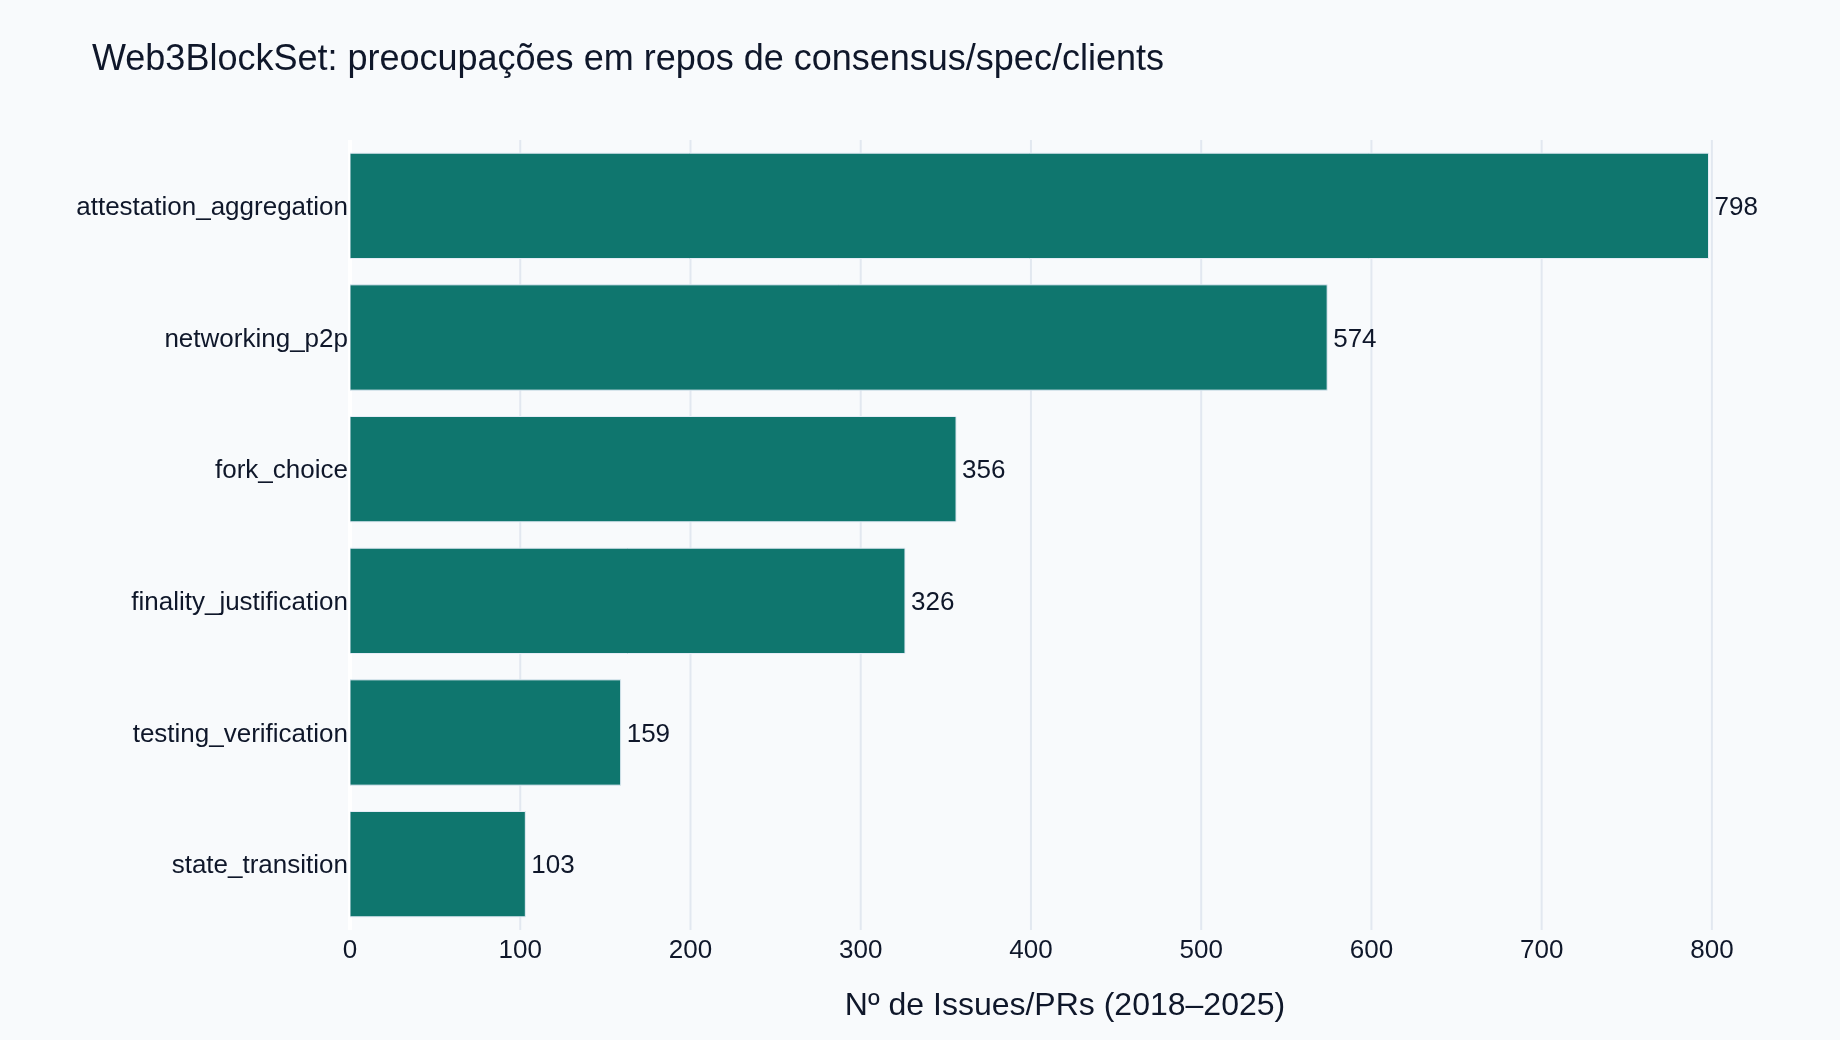
\includegraphics[width=\columnwidth]{figures/fig1_w3_concerns.png}
\caption{Web3BlockSet: Issues/PRs por preocupação em repos de consensus/spec/clients.}
\label{fig:w3}
\end{figure}

\begin{figure}[t]
\centering
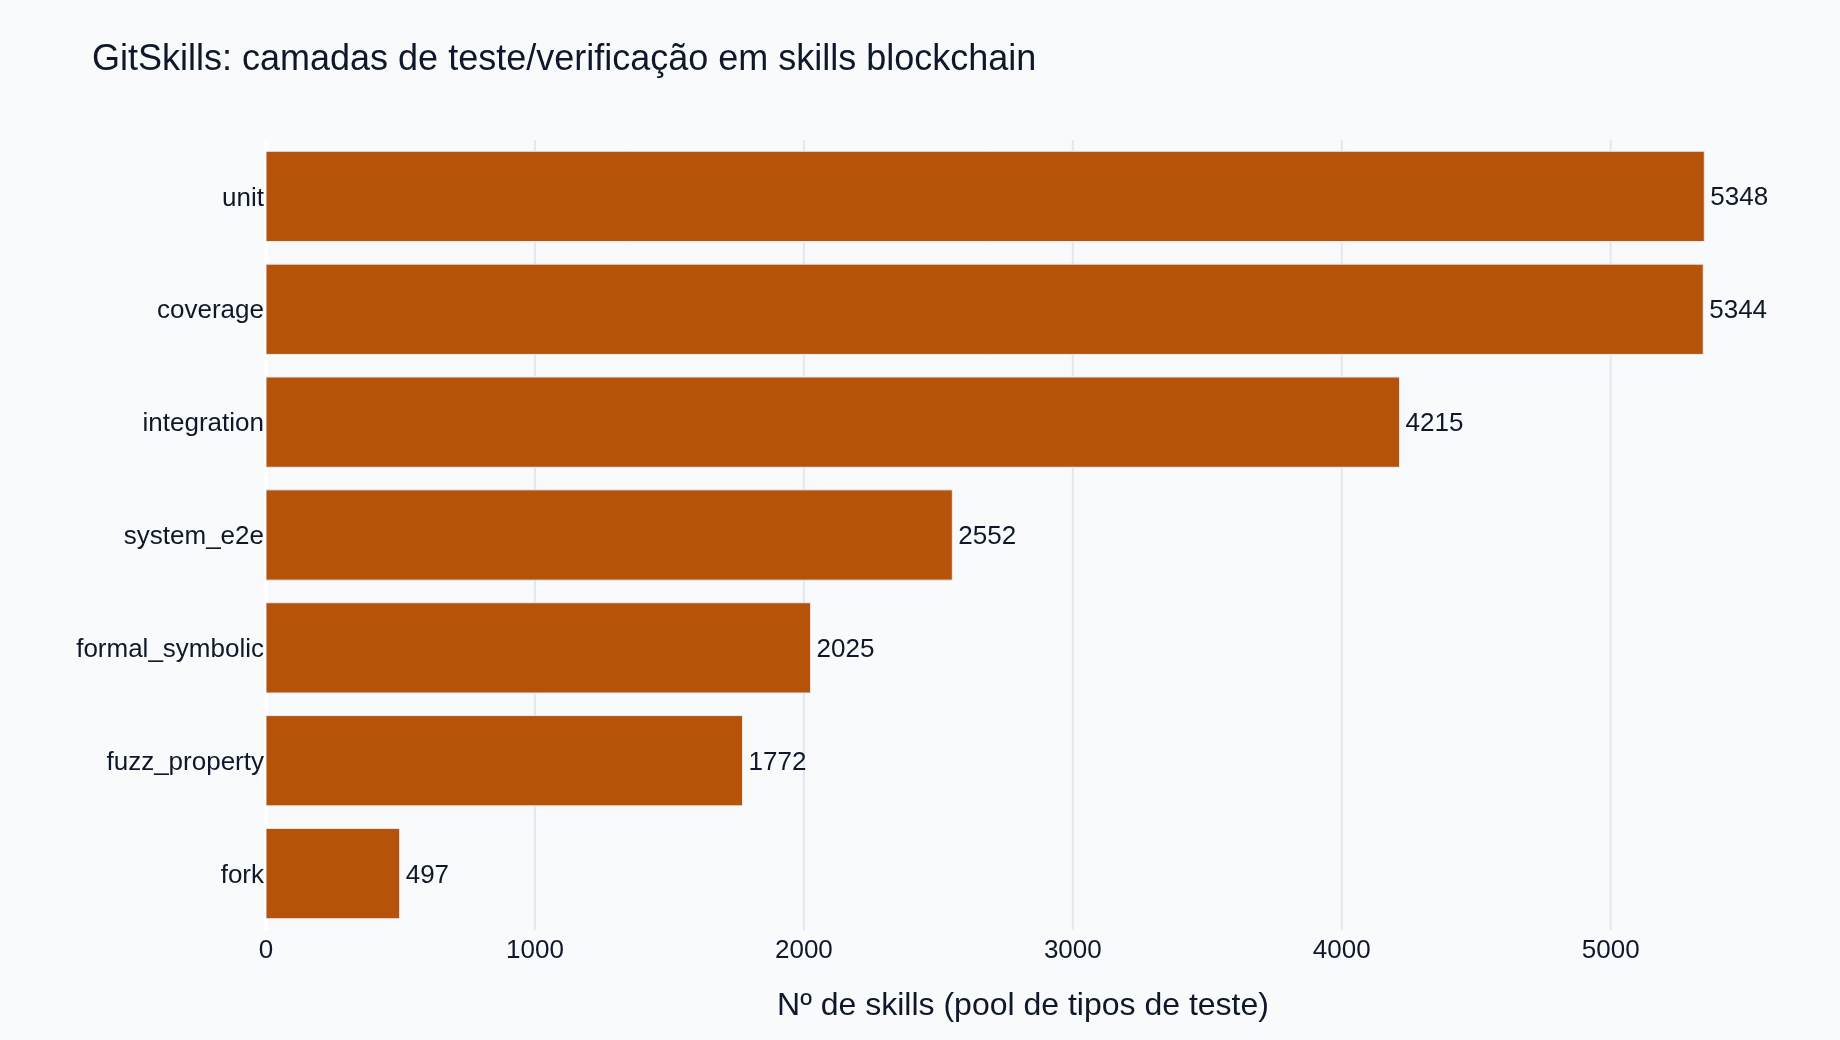
\includegraphics[width=\columnwidth]{figures/fig2_gitskills_layers.png}
\caption{GitSkills: camadas de teste/verificação no pool blockchain.}
\label{fig:layers}
\end{figure}

\begin{figure}[t]
\centering
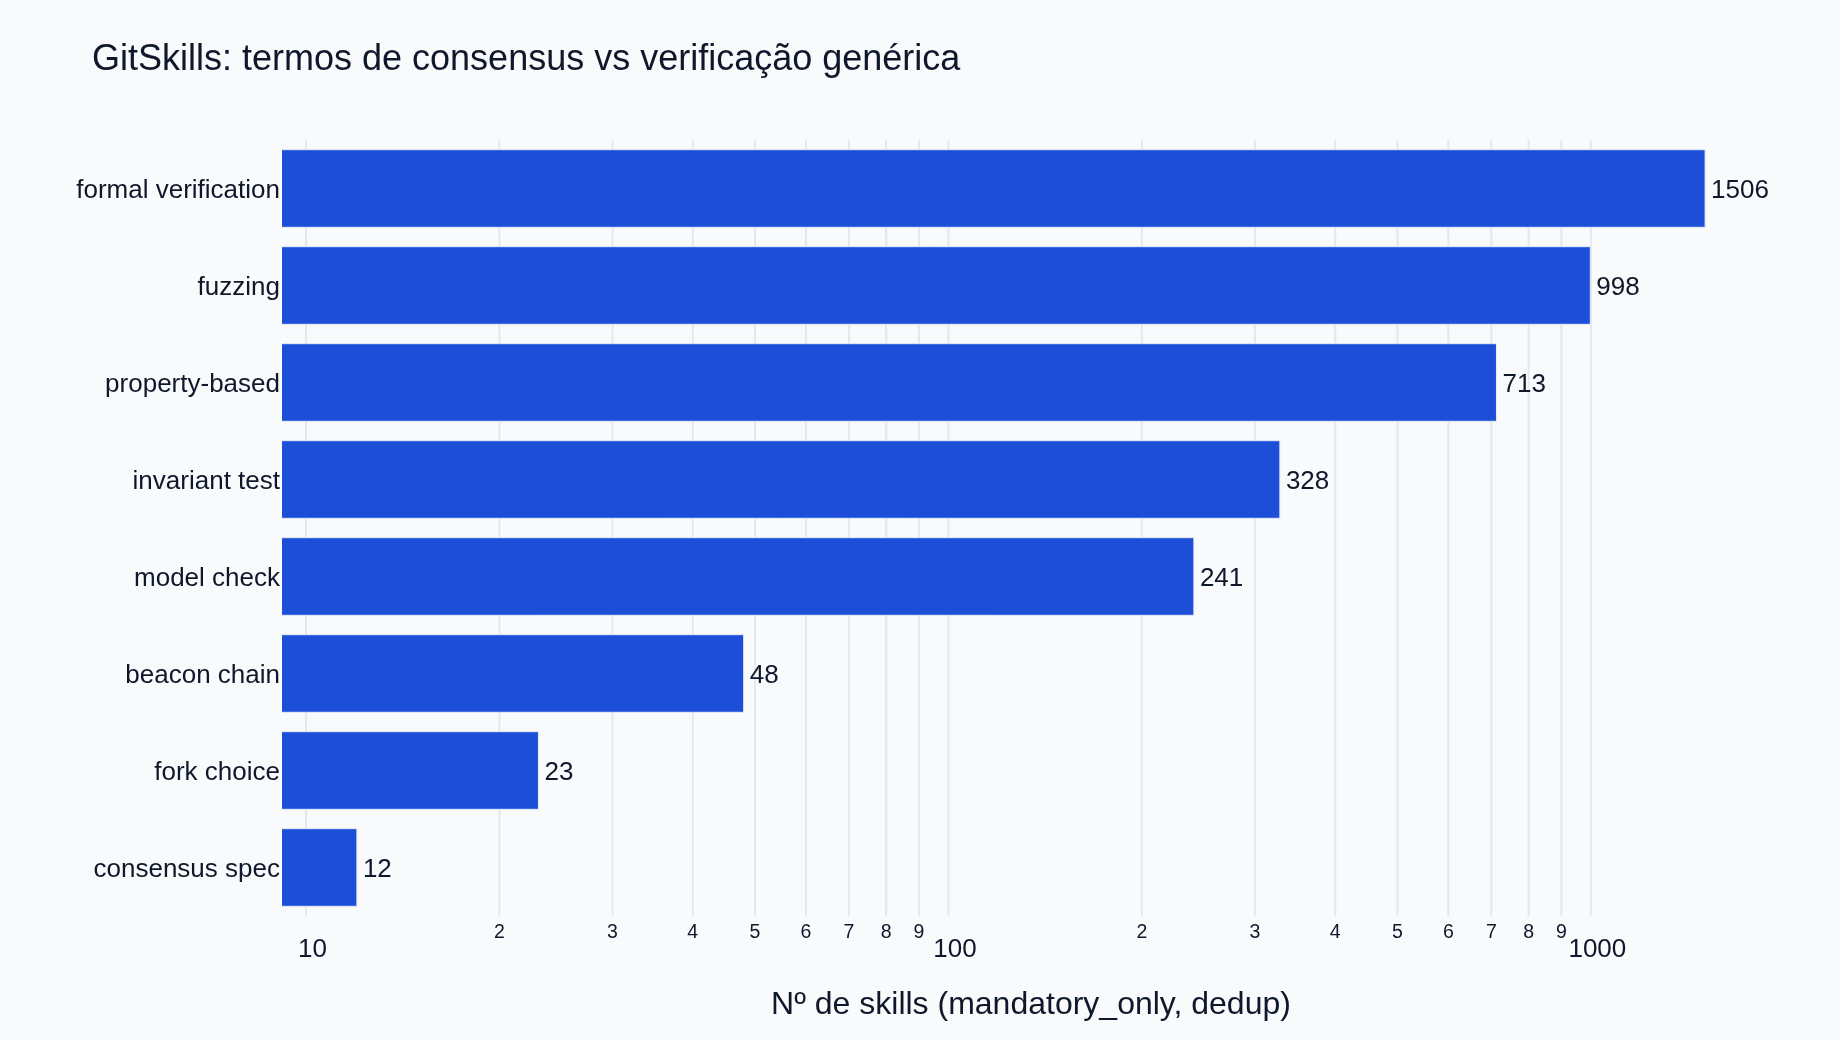
\includegraphics[width=\columnwidth]{figures/fig3_gitskills_terms.png}
\caption{GitSkills: termos de consensus (raros) vs verificação genérica (frequentes). Eixo~X em escala log.}
\label{fig:terms}
\end{figure}

\begin{figure}[t]
\centering
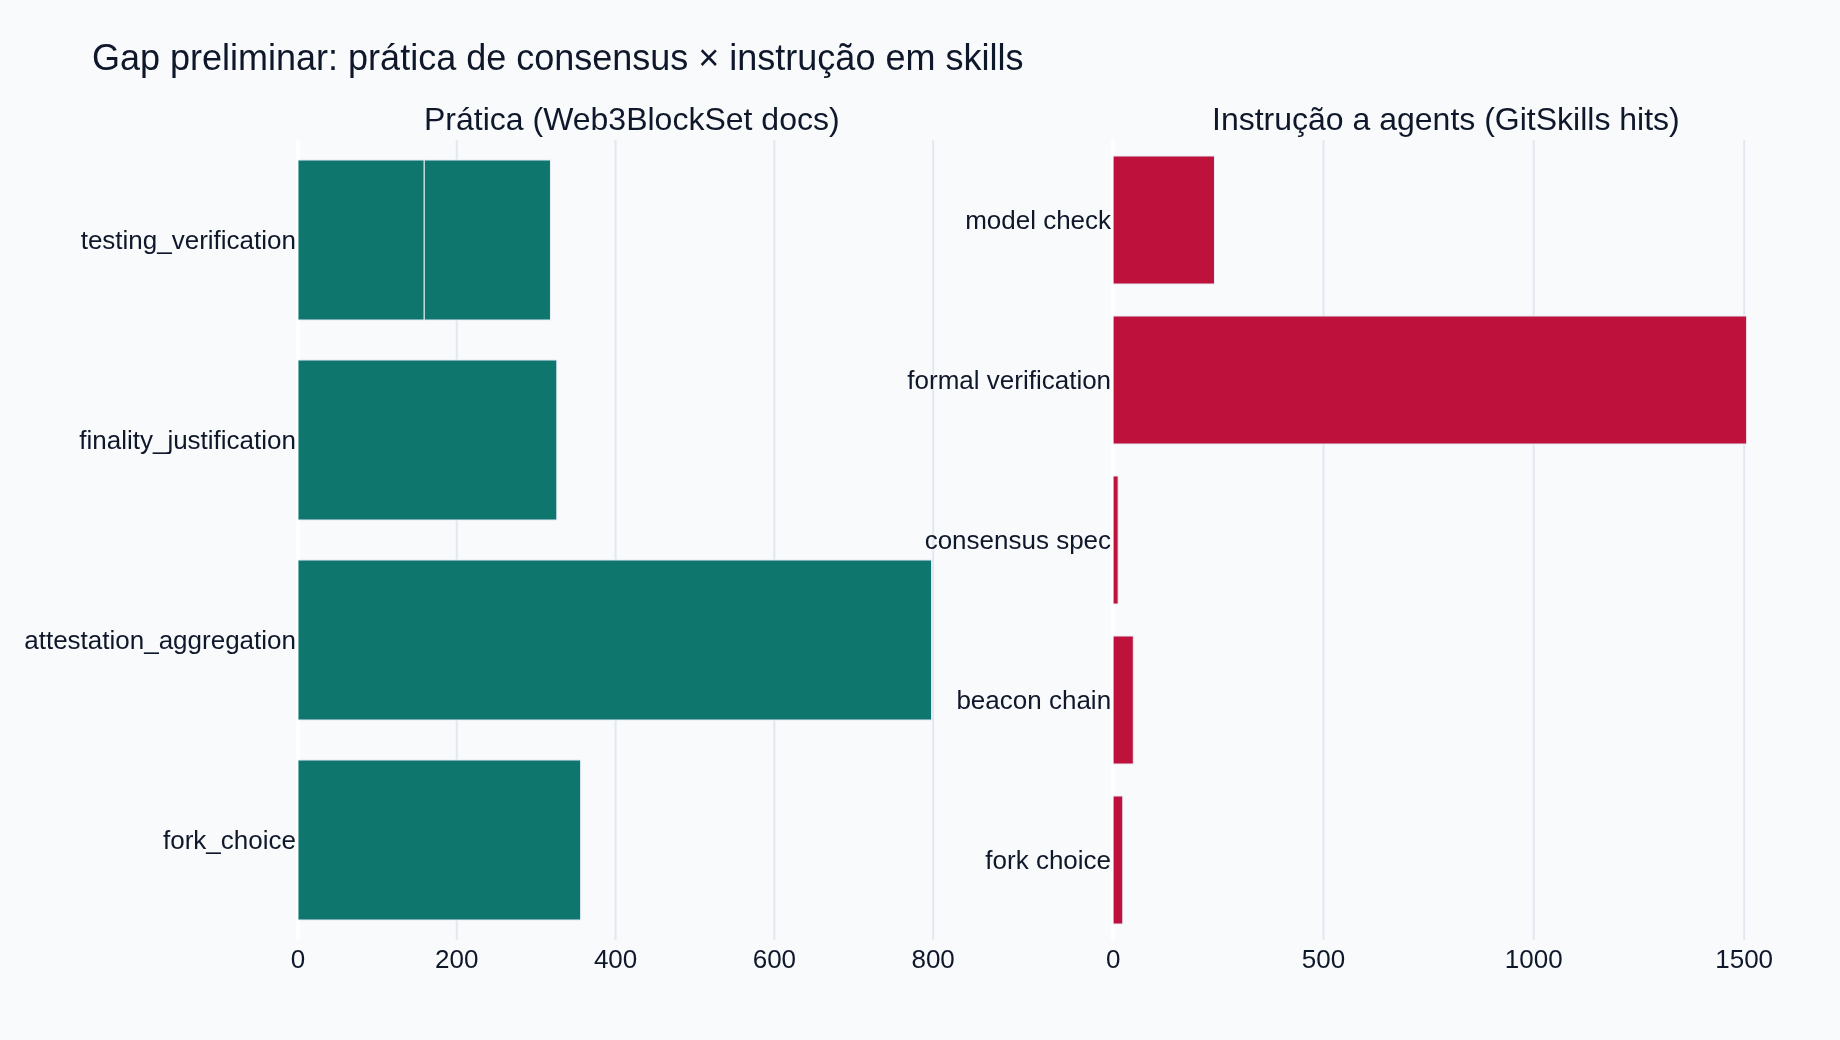
\includegraphics[width=\columnwidth]{figures/fig4_gap.png}
\caption{Gap preliminar lado a lado: prática (docs) vs instrução (skills).}
\label{fig:gap}
\end{figure}

\paragraph{Prática (Web3BlockSet).}
No recorte (6 repositórios seed; $N{=}10{.}962$ Issues/PRs em 2018--2025), os buckets de domínio dominam as menções explícitas de testing/verification no texto: attestation (798), networking (574), fork choice (356), finality (326), contra apenas 159 documentos no bucket \texttt{testing\_verification} (Figura~\ref{fig:w3}). Isso \emph{não} implica ausência de testes nos clients; implica que a conversa observável gira em torno de \textbf{componentes da spec}.

\paragraph{Instrução (GitSkills).}
No pool de 17.847 skills com orientação de teste, unit (5.348) e coverage lideram; fork aparece em apenas 497 skills. formal\_symbolic (2.025) e fuzz\_property (1.772) existem, porém os termos específicos de consensus são escassos nas skills distintas: ``fork choice''~=~23, ``consensus spec''~=~12, ``beacon chain''~=~48, contra ``formal verification''~=~1.506 (Figuras~\ref{fig:layers}--\ref{fig:terms}).

\paragraph{Gap (provocação).}
A Figura~\ref{fig:gap} resume o desalinhamento: a prática nomeia \emph{onde} a correção importa (fork choice, attestations, finality); as skills nomeiam \emph{que} família de técnica usar (formal verification, unit tests), com pouca rastreabilidade a cláusulas do consensus spec. Numericamente, o contraste é gritante na cauda semântica (Tabela~\ref{tab:gap}): dezenas de skills citam ``fork choice'', enquanto centenas de Issues/PRs do recorte discutem o tema; milhares de skills citam ``formal verification'', enquanto o bucket textual de testing/verification na prática é o menor entre os buckets de domínio. Para um WIP, isso motiva a hipótese central:

\begin{table}[t]
\caption{Proxies do gap (unidades distintas; interpretação qualitativa).}
\label{tab:gap}
\centering
\scriptsize
\begin{tabular}{@{}lrr@{}}
\toprule
Sinal & Prática (docs) & Skills (hits) \\
\midrule
fork choice / bucket & 356 & 23 \\
beacon / attestation proxy & 798 & 48 \\
consensus spec term & --- & 12 \\
testing\_verification bucket & 159 & --- \\
``formal verification'' & --- & 1\,506 \\
``model check'' & --- & 241 \\
\bottomrule
\end{tabular}
\end{table}

\begin{quote}
\emph{Agents hoje recebem instruções de verificação desalinhadas da ontologia do consensus Ethereum; fechar esse gap exige agentes que liguem cláusula/Issue $\rightarrow$ propriedade $\rightarrow$ oráculo/teste.}
\end{quote}

\section{Por que isso importa (e como conecta a BMC/agents)}

\subsection{Implicações}
\begin{itemize}
\item \textbf{Para agents de verificação:} tradutores de spec precisam de um backlog empírico de propriedades---Issues/PRs são uma fonte rastreável e versionável.
\item \textbf{Para BMC / model checking de specs:} propriedades sem âncora na prática viram exercícios; propriedades sem engine viram wishlist. O WIP posiciona a âncora empírica \emph{antes} da engenharia do checker.
\item \textbf{Para teste gerado por agentes:} suites ``traceable to specification clauses''~\cite{consensusSpecs} exigem exatamente o elo que o gap sugere estar fraco nas skills atuais.
\item \textbf{Para pesquisa MSR / Mining Challenge:} demonstra valor em cruzar datasets de \emph{instrução a agents} (GitSkills) com datasets de \emph{prática} (Web3BlockSet) no mesmo domínio crítico.
\item \textbf{Para formação em FV:} oferece um caminho de entrada sem exigir, no curto prazo, expertise em SMT---mas exige aprender a falar a língua de propriedades (safety/liveness/reachability).
\end{itemize}

\subsection{Atenções (não overclaim)}
Matching lexical é proxy; ``formal verification'' em skills pode ser shallow; Issues misturam suporte e manutenção; EIPs ampliam o recorte além de consensus puro; GitSkills e Web3BlockSet têm unidades incomparáveis (skills vs docs)---comparamos padrões, não taxas absolutas. A ausência de um termo em skills não prova ausência de conhecimento do autor da skill.

\subsection{Remediações e agenda (4 frentes)}
\begin{enumerate}
\item \textbf{Agora (este WIP):} concluir anotação cega $\rightarrow$ backlog de propriedades esboçadas com evidência verbatim.
\item \textbf{Curto prazo:} agent piloto Issue/cláusula $\rightarrow$ propriedade em template (safety/liveness) + citação da seção do \texttt{consensus-specs}.
\item \textbf{Médio prazo:} ligar propriedades a testes existentes do consensus-specs / clients (rastreabilidade).
\item \textbf{Longo prazo (fora do short):} traduzir um subconjunto para BMC (p.ex., frontend Python / ESBMC)---aprendizado dirigido alinhado à oportunidade de research assistant, não claim deste artigo.
\end{enumerate}

\section{Exemplos de esboços de propriedade (ilustrativos)}

Sem validação completa ainda, esboçamos o tipo de saída que a anotação cega deve produzir---útil tanto para o paper quanto para treinar futuros agents:

\begin{itemize}
\item \textbf{Fork choice / safety:} ``o algoritmo de escolha de head não seleciona um bloco que viole regras de justificação/finalização já observadas.''
\item \textbf{Finality / safety:} ``dois checkpoints conflitantes não podem ambos ser finalizados.''
\item \textbf{Attestation / validity:} ``agregados só incluem attestations com dados consistentes com o estado do epoch.''
\item \textbf{State transition / reachability:} ``a partir de um estado pré-slot válido, \texttt{process\_slots}/\texttt{process\_block} alcança apenas estados que preservam invariantes de balanço/validadores.''
\end{itemize}

Esses templates são propositalmente informais: o WIP defende que \emph{primeiro} se ancora a propriedade na prática e na spec; \emph{depois} se formaliza para um checker.

\section{Posicionamento face a trabalhos e oportunidades}

Este WIP é ortogonal a estudos de DEx/BaaS~\cite{soares2025bcdex} e complementar ao plano de tipologias de teste em GitSkills: aqui o foco não é a pirâmide unit$\rightarrow$e2e em si, e sim o \textbf{descompasso semântico} entre instrução a agents e a ontologia do consensus. Em relação a agendas de bounded model checking para specs Ethereum~\cite{clarke2018bmc,consensusSpecs}, contribuímos a etapa \emph{upstream}: evidência de quais componentes e falhas a comunidade discute, e quão pouco isso aparece nomeado nas skills. Não reivindicamos implementação de frontend ESBMC neste artigo; reivindicamos um backlog empírico e uma provocação clara para agentes de tradução cláusula$\rightarrow$propriedade---precisamente o tipo de ponte empírica que torna produtiva uma colaboração futura com grupos de systems/software security.

\section{Ameaças à Validade}
\paragraph{Construto.} Keywords e first-match de buckets são proxies; ``formal verification'' em skills pode ser menção superficial.
\paragraph{Interna.} Um documento pode misturar preocupações; atribuímos um único bucket.
\paragraph{Externa.} Seed pequeno de repositórios (sem todos os clients); EIPs alargam o escopo.
\paragraph{Confiabilidade.} Validação manual do esboço de propriedades está em curso ($n$ amostral preparado).

\section{Conclusão}
Cruzando GitSkills e Web3BlockSet, este WIP argumenta que a instrução a agents sobre verificação blockchain está \textbf{desalinhada} da ontologia do consensus Ethereum discutida na prática: muita ``formal verification'' genérica nas skills, pouca menção a fork choice/consensus spec; na prática, o contrário em termos de atenção discursiva a componentes. O valor imediato é um mapa de gap e um protocolo para propriedades candidatas; o valor estratégico é preparar a ponte empírica para agentes e engines de verificação de specs---sem fingir que mining substitui model checking.

\section*{Disponibilidade}
Artefatos em \texttt{2027\_short\_paper\_bridge}; dados-base Web3BlockSet~\cite{soares2026web3blockset} e GitSkills~\cite{gitskills2026}.

\bibliographystyle{IEEEtran}
\bibliography{references}

\end{document}
